\documentclass[fleqn, xcolor=x11names]{beamer}
\usetheme{MyAmsterdam} %тема\
\usecolortheme{default}
\usepackage[utf8]{inputenc}
\usepackage[russian]{babel}
\usepackage[OT1]{fontenc}
\usepackage{amsmath}
\usepackage{amsfonts}
%\usepackage{amssymb}
\usepackage{hyperref}
\usepackage{graphics, graphicx}
\usepackage{color}
\usepackage{enumerate}

% \usepackage{citehack} 
\usepackage{pgfplots}
\usepackage{tikz}
\usetikzlibrary{patterns}

\usepackage{minted}
\usemintedstyle{default}
%my package
\graphicspath{{../figures/}}

\setbeamertemplate{navigation symbols}{} % отключить навигационные значки
\setbeamertemplate{footline}{%
    \hspace{0.94\paperwidth}%
    \usebeamerfont{title in head/foot}%
    \insertframenumber\,/\,\inserttotalframenumber%
} % переопределить нижнуюю панель, убрать всё кроме номера слайда


%\usefonttheme[onlylarge]{structurebold} % названия и текст в колонтитулах выводится полужирным шрифтом.
\usefonttheme[onlymath]{serif}  % привычный шрифт для математических формул
%\setbeamerfont*{frametitle}{size=\normalsize,series=\bfseries} % шрифт заголовков слайдов
\usepackage[nopar]{lipsum} %для генерации большого текста


\newminted[pcode]{python}{baselinestretch=1, fontsize=\small}
\newmintinline[pinline]{python3}{baselinestretch=1}
\definecolor{bg}{rgb}{0.95,0.95,0.95}
%\newminted[lcode]{latex}{baselinestretch=1, bgcolor=bg}
\newmintinline[linline]{latex}{baselinestretch=1}

\usepackage{tcolorbox}
\tcbuselibrary{minted,skins}

\newtcblisting{lcode}{
    listing engine=minted, %use minted for highlight
    colback=lcodebg, %background color
    colframe=black!50, %width of frame
    listing only,
    minted style=colorful,
    minted language=latex,
    minted options={linenos=false,texcl=true}, %lines - number of lines
    left=1mm,
}
\definecolor{lcodebg}{rgb}{0.95,0.95,0.95}


\usepackage{tikz}
\usetikzlibrary{arrows,positioning}
\usepackage{listings}
\lstset{language=Python}

\newcommand{\real}{\mathbb{R}}
\newcommand{\norm}{\mathop{\rm norm}\limits}
\newcommand{\softmax}{\mathop{\rm softmax}\limits}

\definecolor{beamer@blendedblue}{rgb}{0.037,0.366,0.75}

\title{\bfseries График в параллельных осях}
\author[Тыцкий В.И.]{Студент: Тыцкий В.И.\\[1ex]  {\small Научный руководитель: Майсурадзе А.И.}}
\institute[ВМК МГУ]{МГУ имени М. В. Ломоносова, факультет ВМК, кафедра ММП}
\date{}

\begin{document}

\begin{frame}
\titlepage
\end{frame}

\begin{frame}{Примеры диаграмм}
    \centering
    \begin{tabular}{cc}
        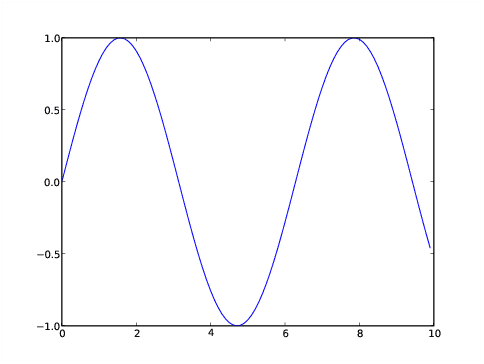
\includegraphics[width=4cm]{example_1.png} &
         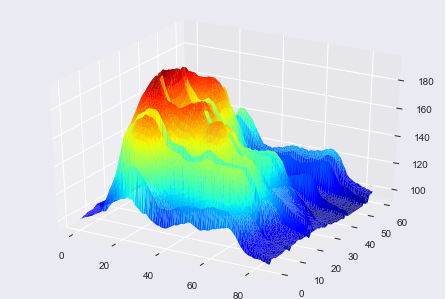
\includegraphics[width=4cm]{example_2.png} \\
         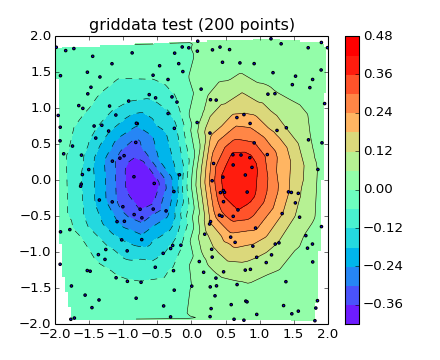
\includegraphics[width=4cm]{example_3.png} &
         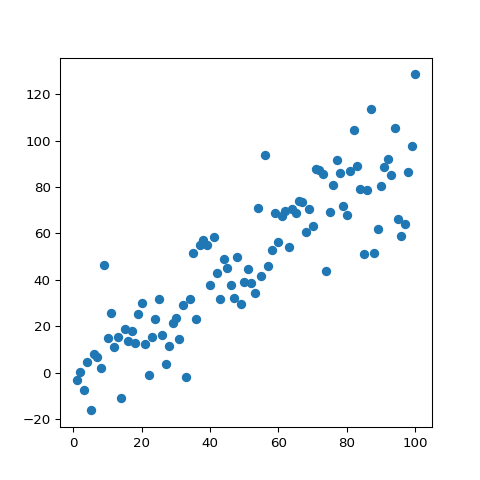
\includegraphics[width=4cm]{example_4.png} 
    \end{tabular}       
\end{frame}

\begin{frame}{Классический график в параллельных осях}
    \begin{figure}[htb]
        \centering
        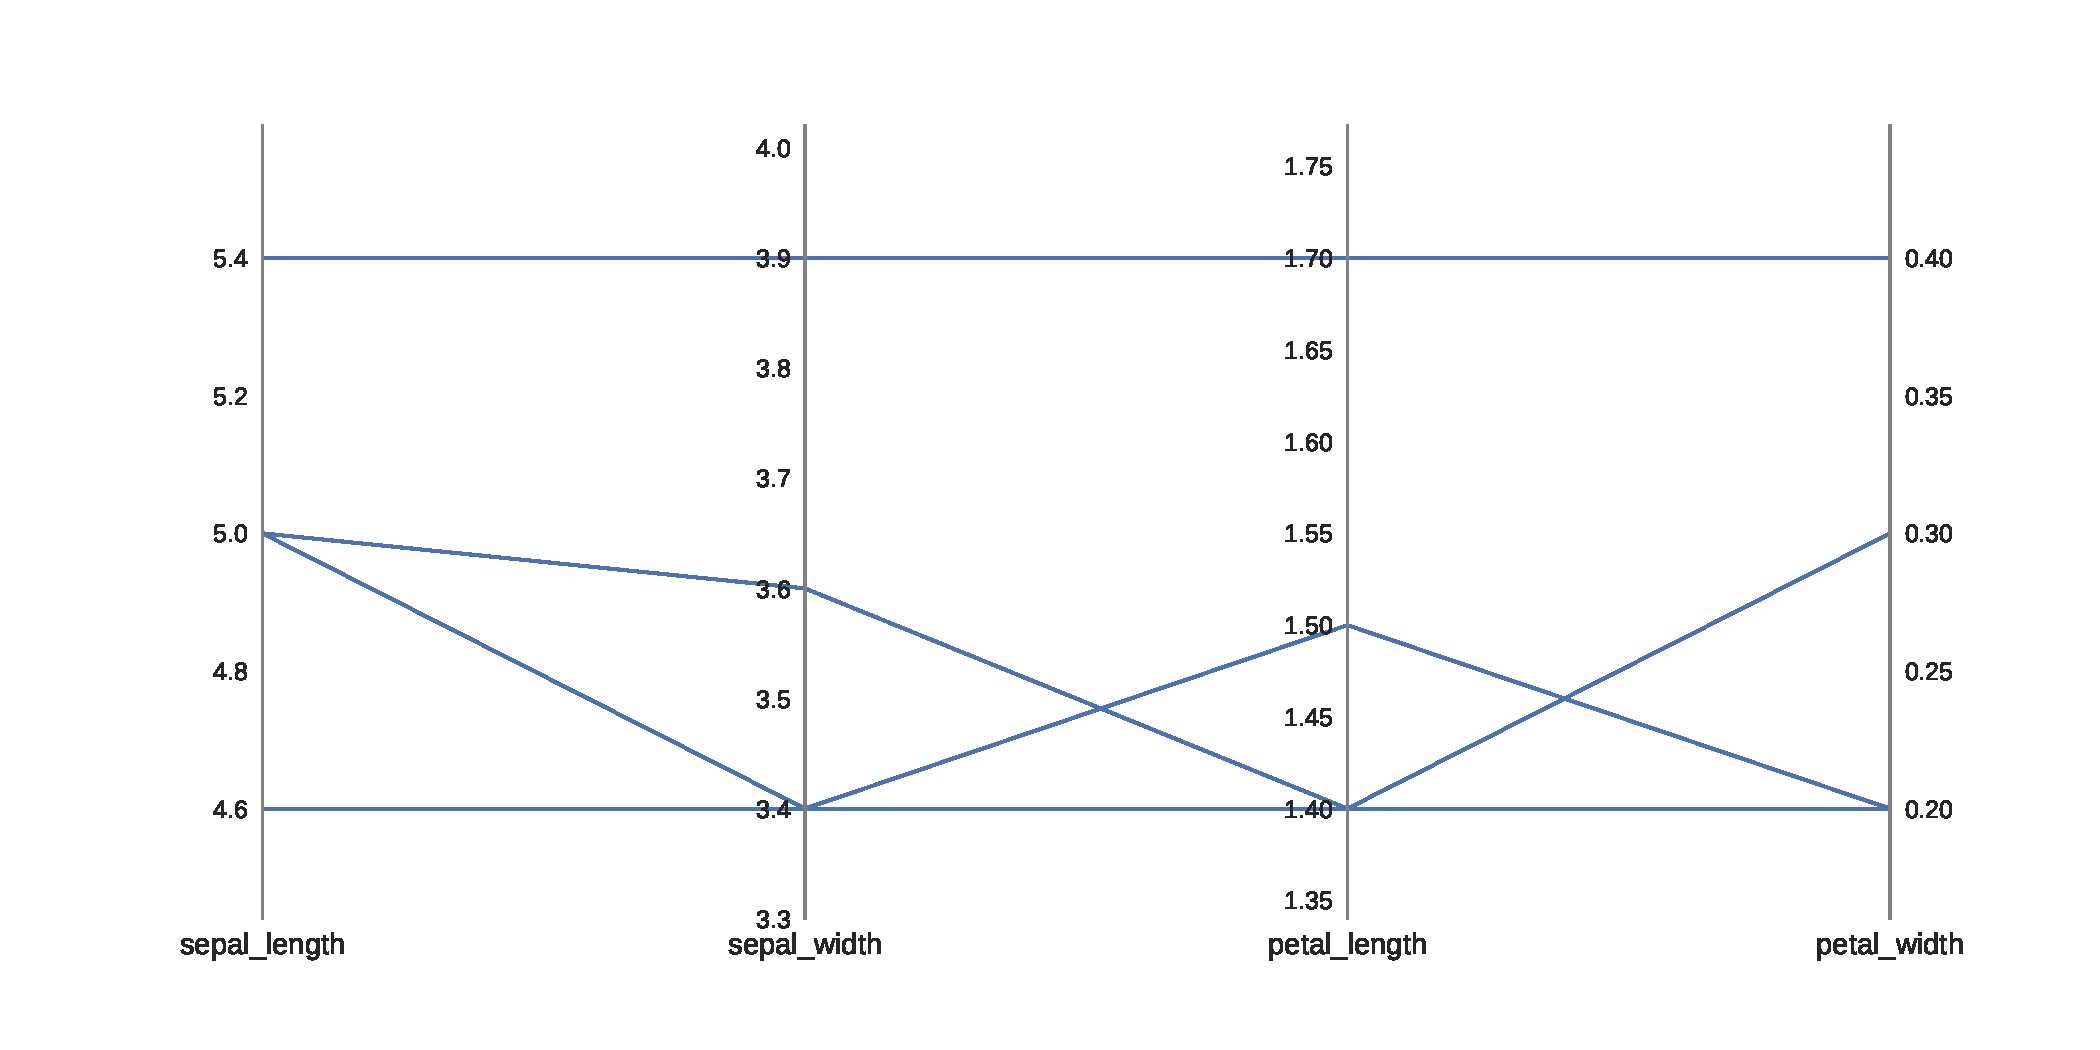
\includegraphics[width=10.5cm]{classic_pc.pdf}
    \end{figure}
\end{frame}

\begin{frame}{Естественные вопросы при построении}
    \begin{itemize}
        \item В каком порядке расположить оси?
        \item В какую сторону направлять оси?
        \item Какой масштаб выбрать для каждой оси?
    \end{itemize}
\end{frame}


\begin{frame}{Модификации: кластеры}
    \begin{figure}[htb]
        \centering
        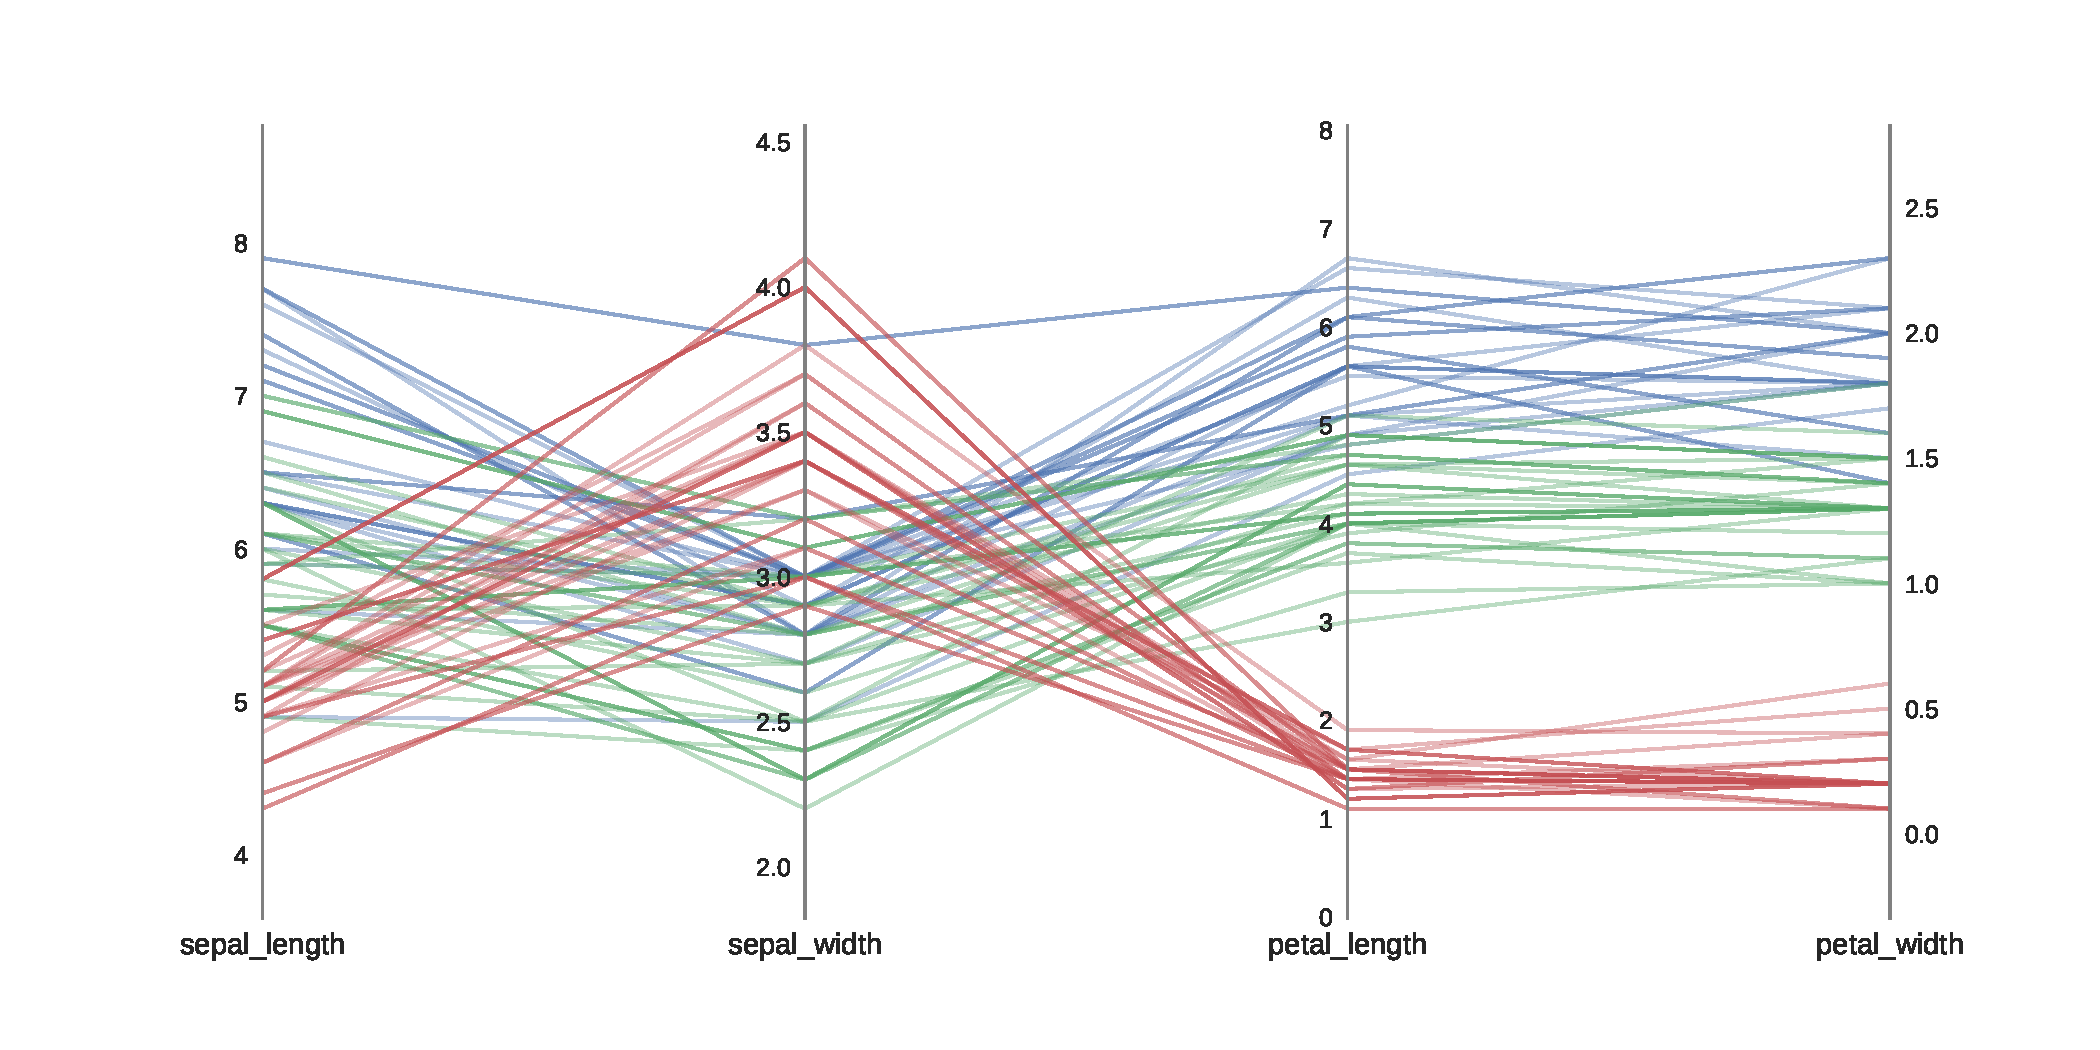
\includegraphics[width=10.5cm]{color_pc.pdf}
    \end{figure}
    Чаще всего именно в таком виде используют график в параллельных осях.
\end{frame}

\begin{frame}{Модификации: сглаживание линий}
    \begin{figure}[htb]
        \centering
        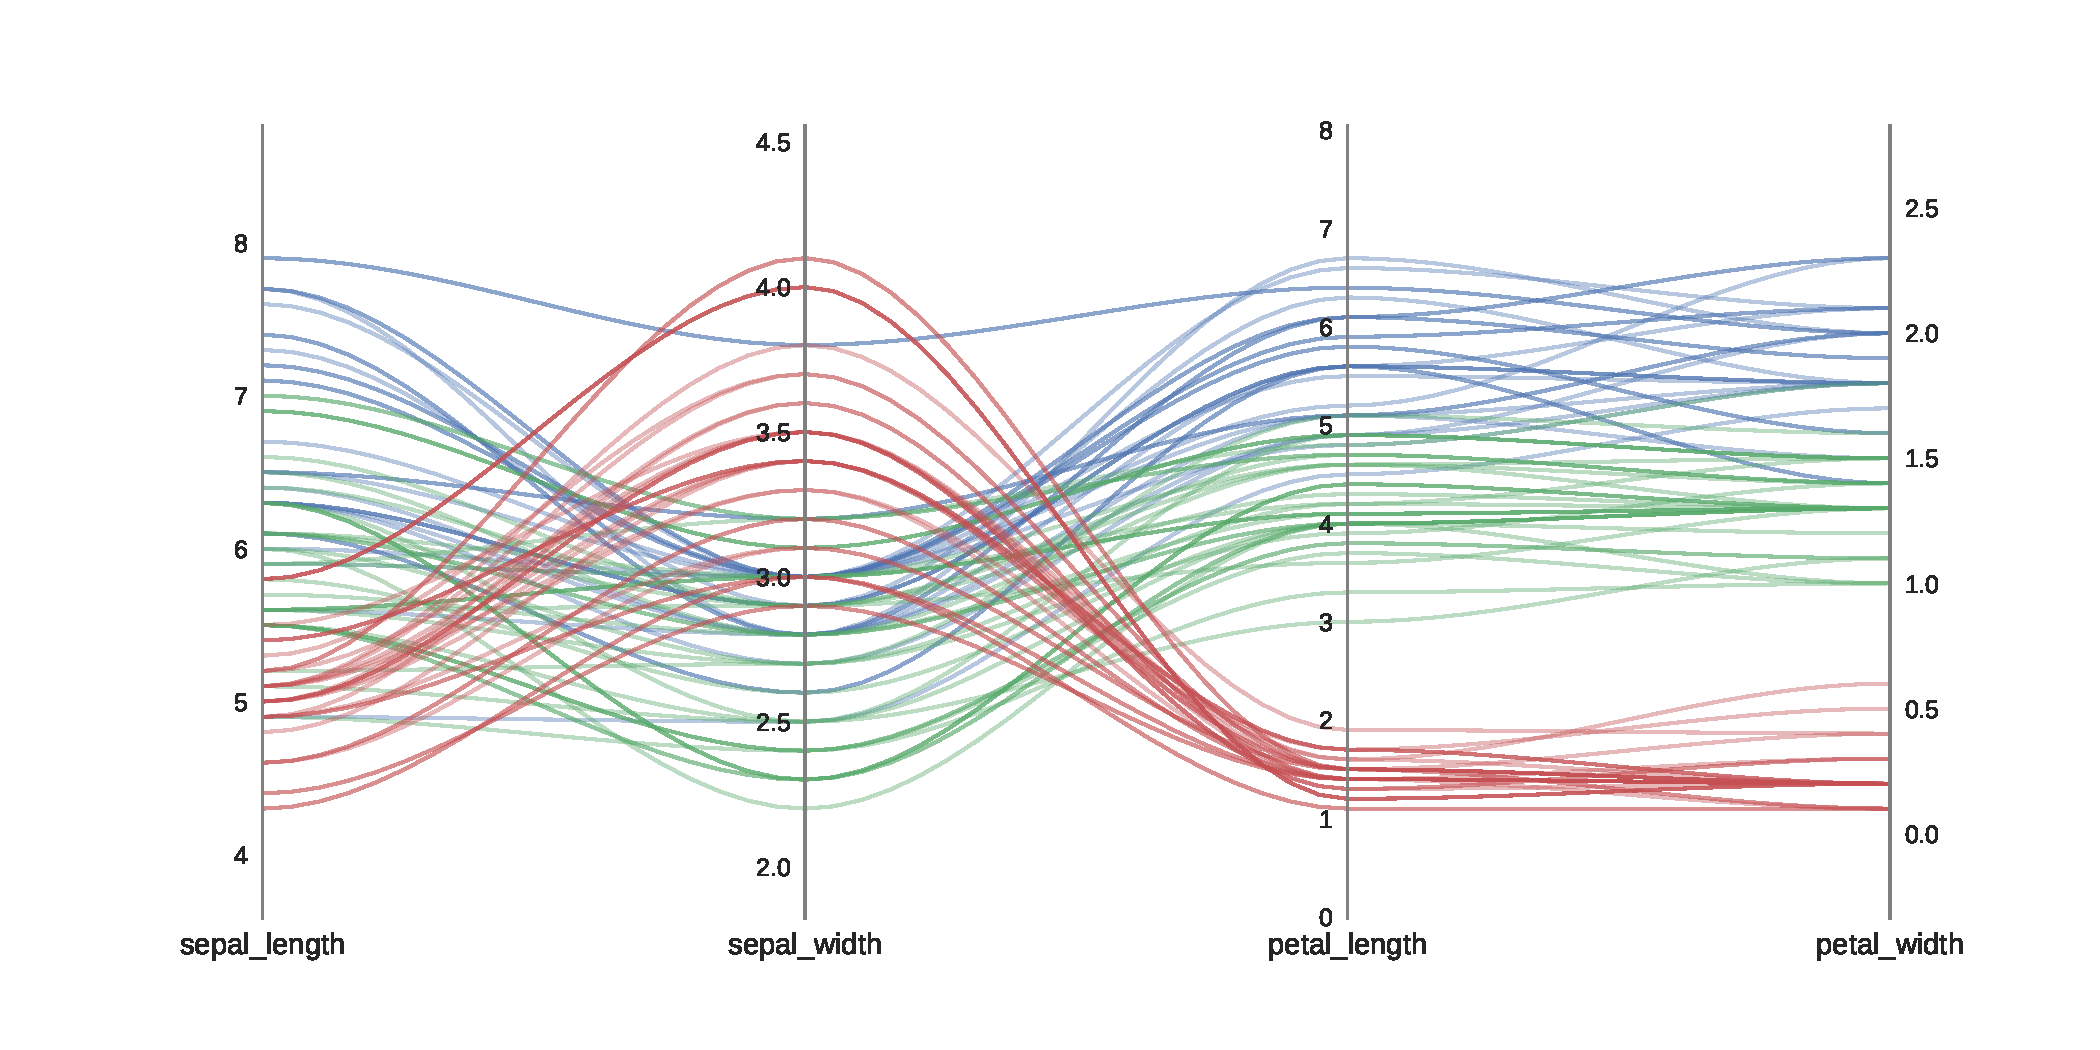
\includegraphics[width=10.5cm]{smooth_pc.pdf}
    \end{figure}
    Человеку проще воспринимать гладкие линии, поэтому читаемость графика заметно возрастает.
\end{frame}

\begin{frame}{Модификации: связывание линий}
    \begin{figure}[htb]
        \centering
        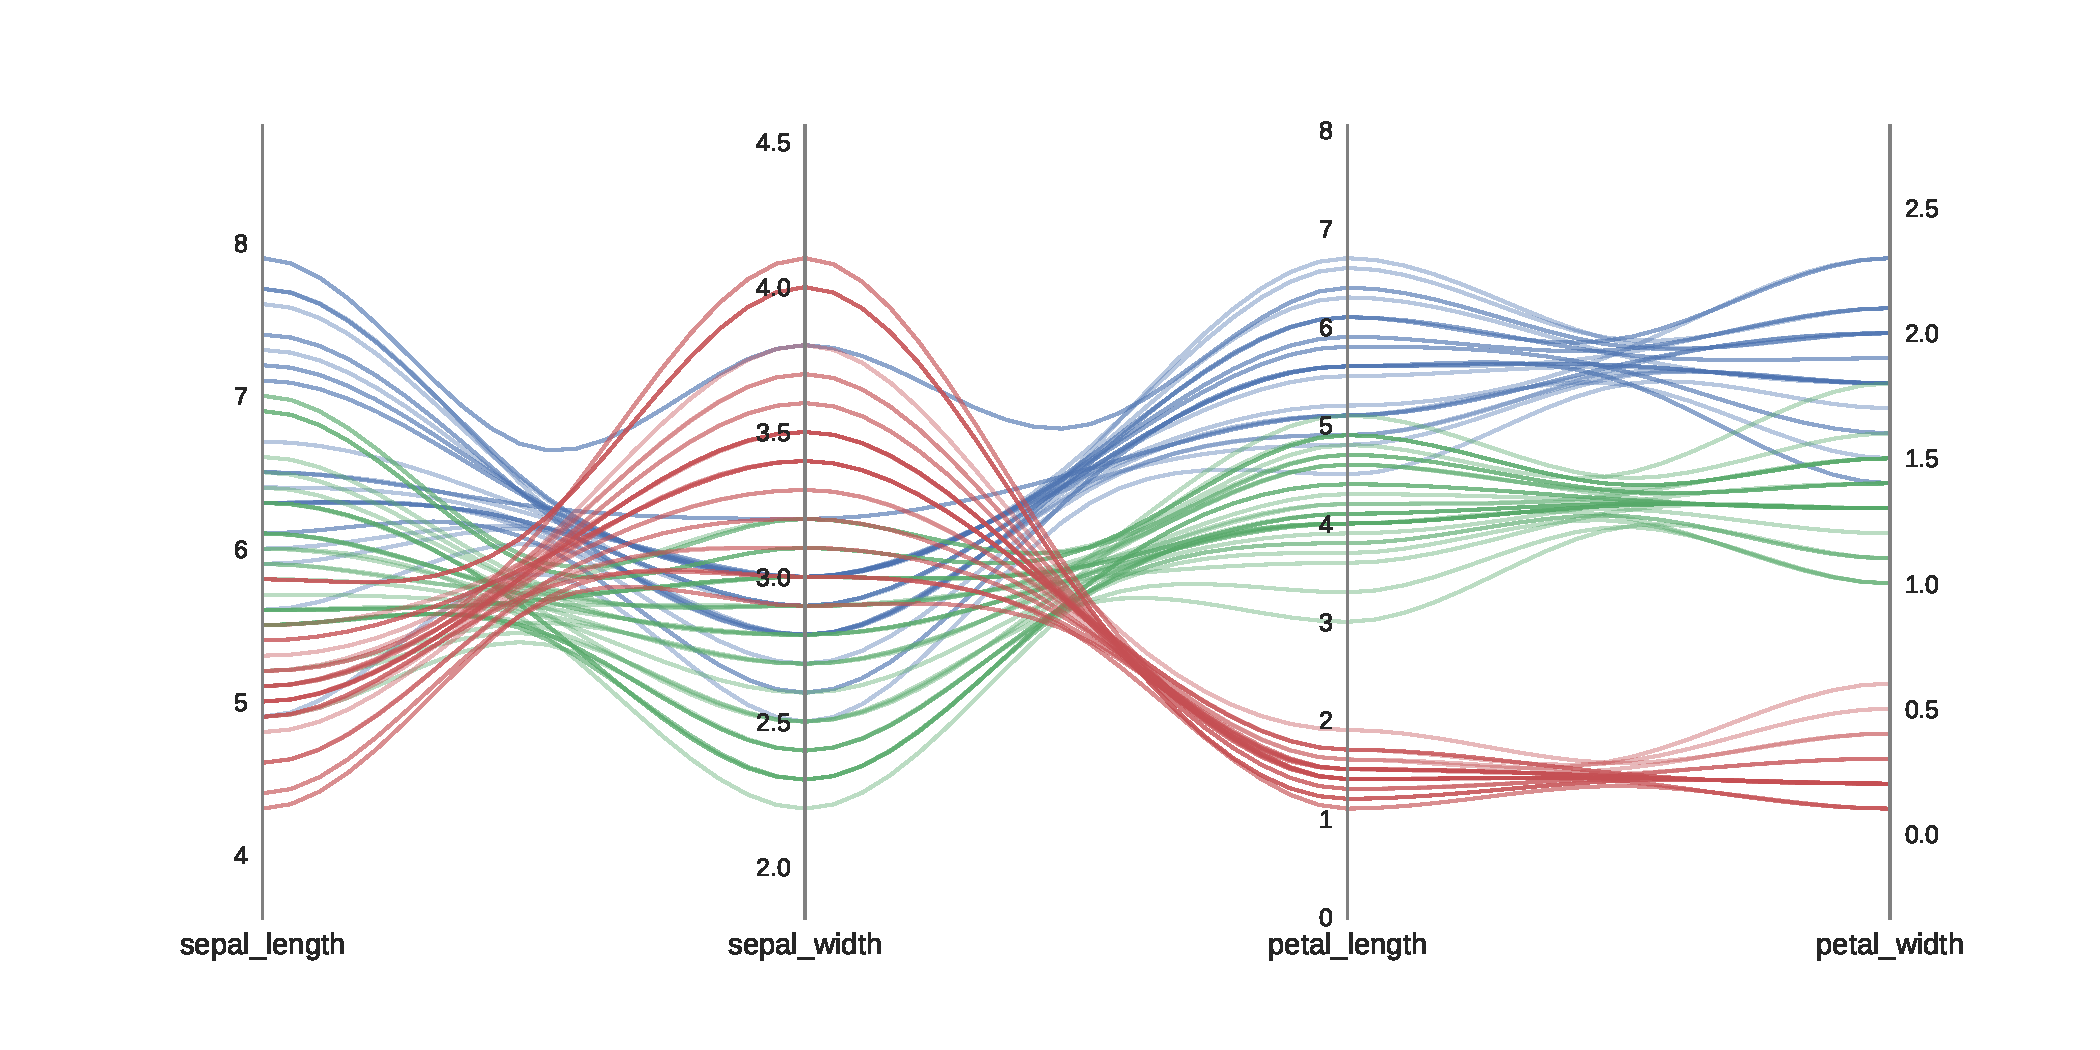
\includegraphics[width=10.5cm]{bundle_0.3_pc.pdf}
    \end{figure}
\end{frame}

\begin{frame}{Модификации: связывание линий}
    \begin{figure}[htb]
        \centering
        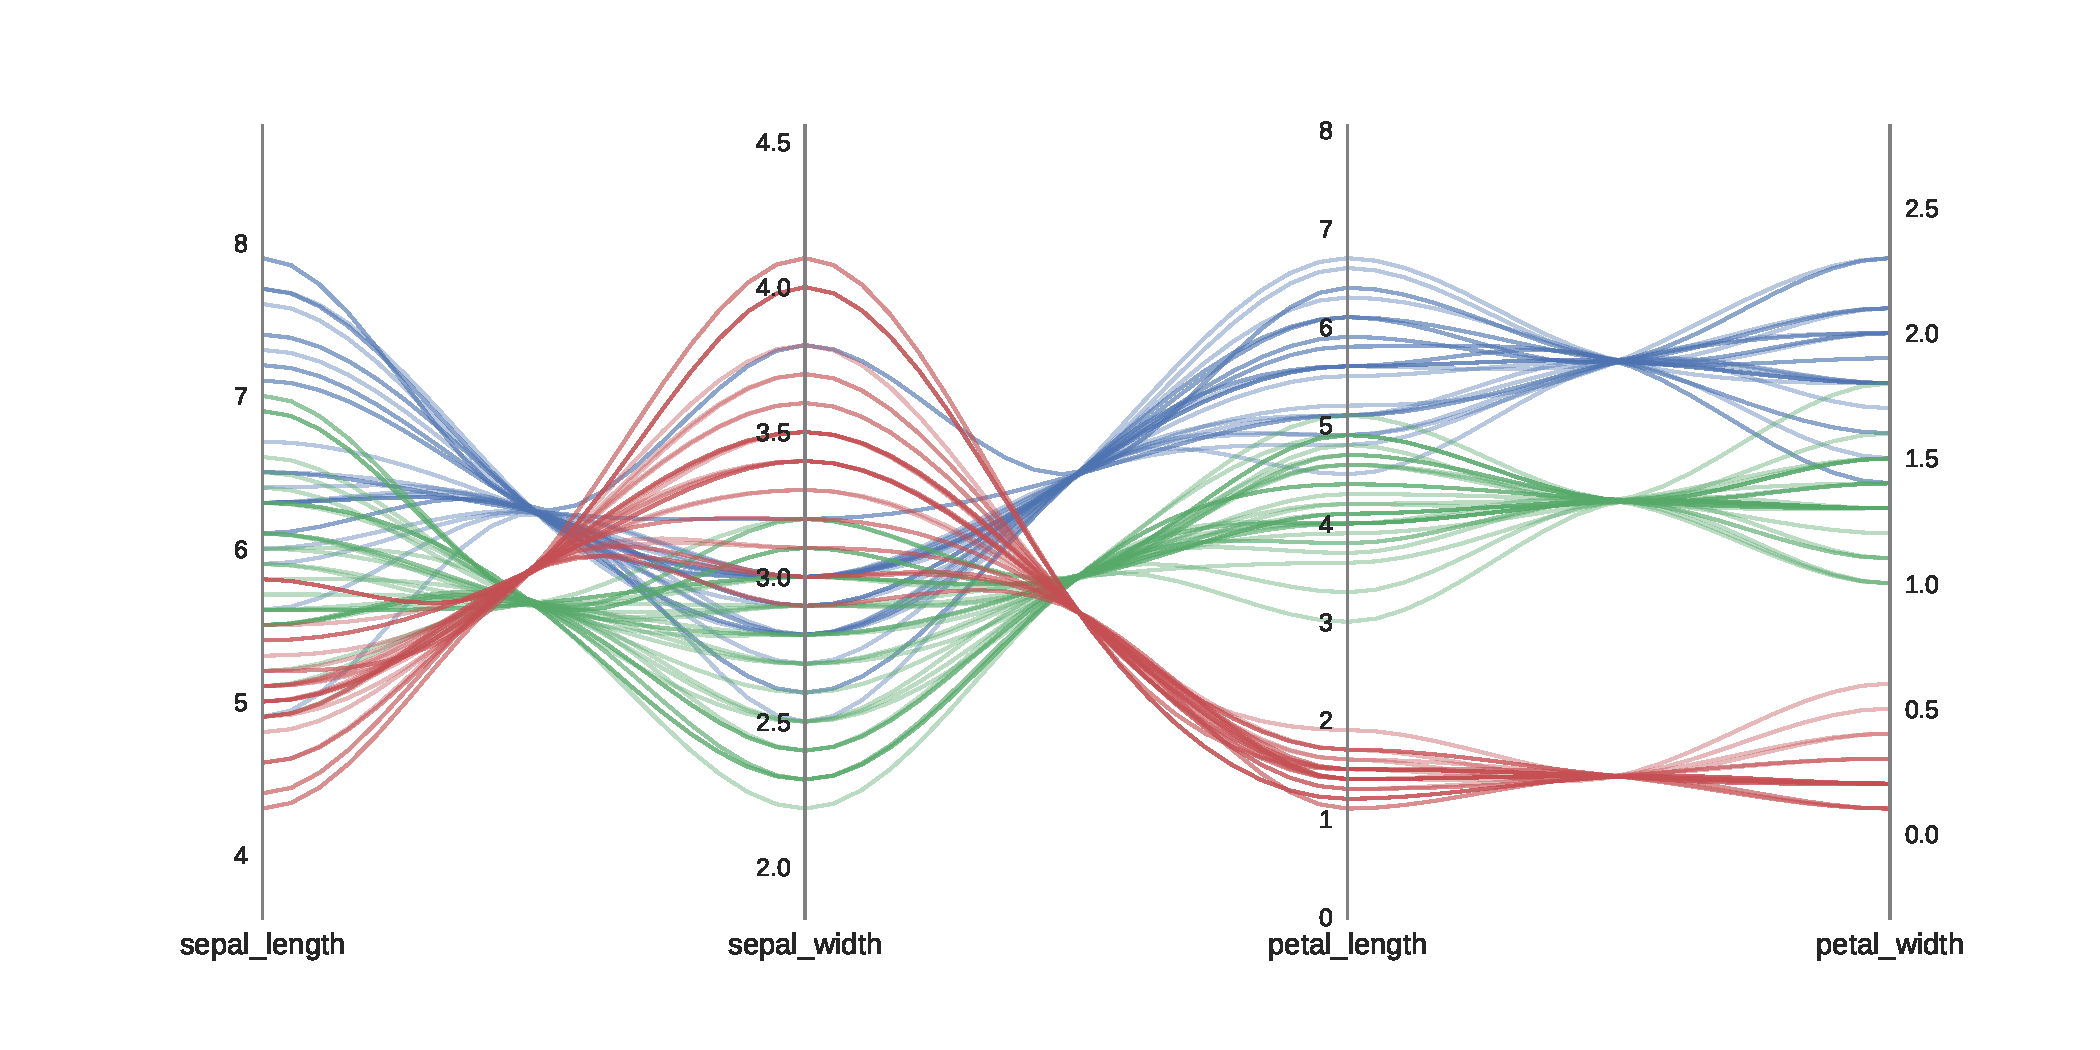
\includegraphics[width=10.5cm]{bundle_0.01_pc.pdf}
    \end{figure}
\end{frame}

\begin{frame}{Модификации: иерархические графики}
    \begin{figure}[htb]
        \centering
        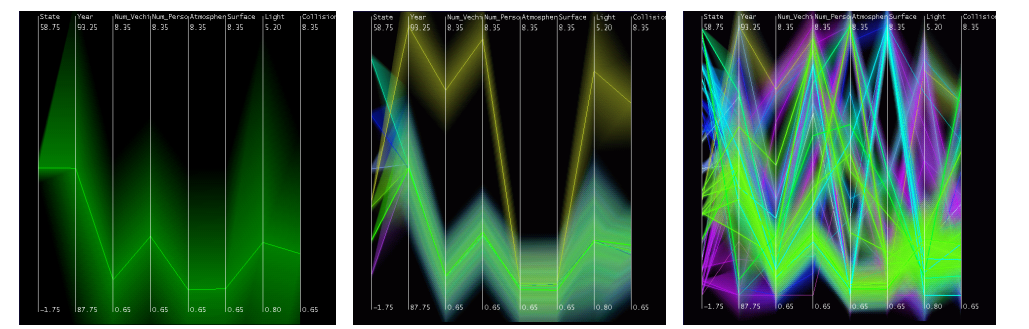
\includegraphics[width=10.5cm]{hierarchical.png}
    \end{figure}
\end{frame}

\begin{frame}{Обзор текущих средств}
    \begin{itemize}
        \item На Python есть простейшая реализация лишь в библиотеке pandas!
        \item ELKI, GGobi, Mondrian, Orange и ROOT.
        \item Parcoords.js интерактивная библиотека на JavaScript.
    \end{itemize}

    \vspace{30px}
    Вывод:
    \begin{itemize}
        \item Необходимо создать свою ''полноценную библиотеку''! \textbf{(исправить это предложение)}
    \end{itemize}

\end{frame}

\begin{frame}{О библиотеке: цели}
    \begin{itemize}
        \item Дать возможность исследователям ''безболезненно'' использовать график 
        в параллелльных осях
        \item Построение красивых и информативных графиков из ''коробки''.
        \item Реализация всевозможных видов данных графиков
    \end{itemize}
\end{frame} 

\begin{frame}{О библиотеке: технические подробности}
    \begin{itemize}
        \item Статические графики.
        \item Библиотека пишется на языке Python на базе matplotilb.       
        \item Простой высокоуровневый интерфейс. Как и в библиотеке seaborn методы могут принимать pandas.DataFrame,
        обычные numpy массивы или списки -- для всего единый интерфейс.
    \end{itemize}
\end{frame}

\begin{frame}{О библиотеке: возможности}
    \begin{itemize}
        \item Построение классических графиков в параллельных осях
        \begin{itemize}
            \item Возможность рисовать гладкие линии.
            \item Возможность ''связывания'' линий кластеров.
            \item Возможность ''связывания'' линий на основе близости. 
        \end{itemize}
        \vspace{10px}
        \item Построение иерархических графиков
        \begin{itemize}
            \item Отрисовка полупрозрачного градиента.
            \item Работа с иерархическими кластерами.
            \item Изображение распределения с помощью градиента.
        \end{itemize}
    \end{itemize}
\end{frame}

\begin{frame}{О библиотеке: дополнительные возможности}
    \begin{itemize}
        \item выделение подмножества линий в  диапазоне значений одной из осей.
        \item нахождение оптимального расположения осей.
        \item создание иерархических кластеров на основе входящей выборки.
    \end{itemize}
\end{frame}

\begin{frame}{Итоги (после первого семестра)}
    \begin{itemize}
        \item Возможность рисовать гладкие линии. \textbf{Пока что не добавлен параметр задающий вид кривой}.
        \item Возможность ''связывания'' линий кластеров. 
        Добавлен непрерывный параметр задающий степень связывания.
        \item \textbf{Возможность связывания линий на основе близости не реализована}
        \item Интерфейс для пользователя практически полностью повторяет реализацию seaborn.\footnote{
            Большинство графиков в презентации нарисованы с помощью данной библиотеки.}
    \end{itemize}
\end{frame}
\end{document}